
\chapter{Results}


\section{The optimal solution}
Before starting any MGA studies, it is important to investigate and understand the optimal solution of the problem at hand. In this section, the found optimal solutions of the model will be presented. A range of CO2 constraints have been investigated, and as the CO2 constraint is altered a new optimal solution is found, therefore four optimal solutions representing a business as usual scenario, a 50\% CO2 reduction, a 80\% CO2 reduction and a 95\% CO2 reduction scenario will be presented. 

\begin{figure}[h]\centering
	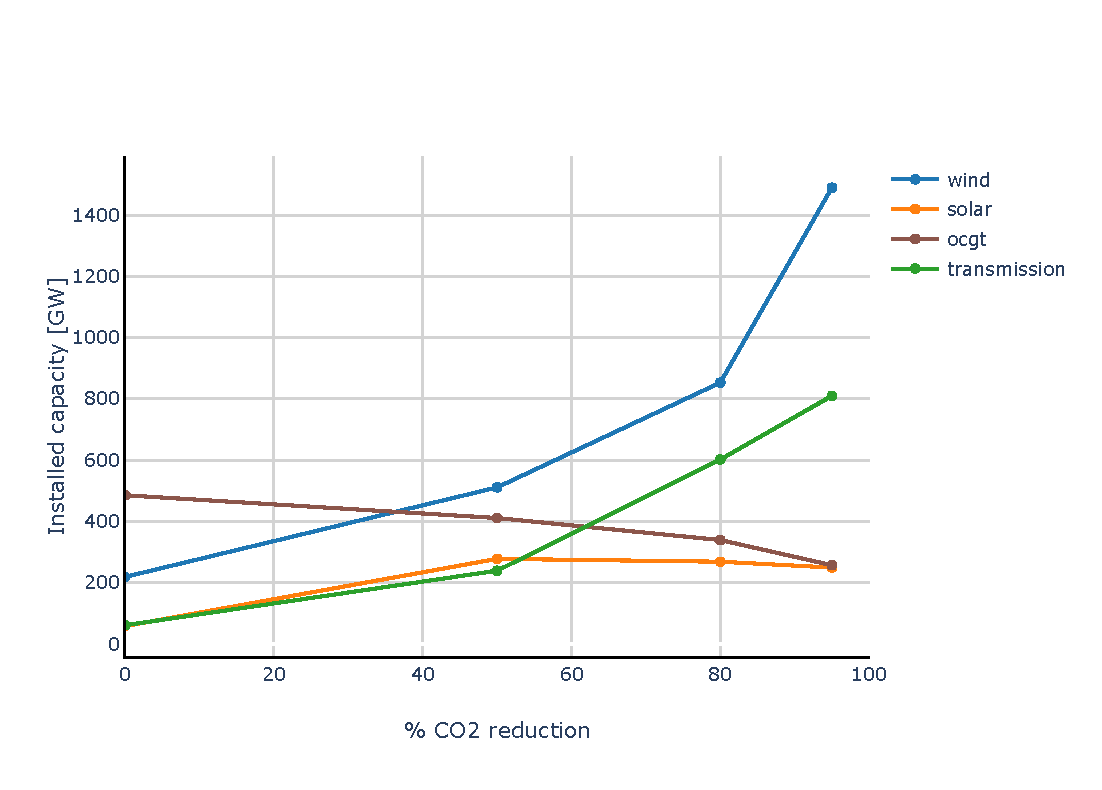
\includegraphics[width=1.\textwidth]{./Images/optimal_solutions_summary}
	\caption{Optimal solutions }
	\label{fig:Optimal_Solutions_summary}
\end{figure}

On figure \ref{fig:Optimal_Solutions_summary}, the summarized technology capacities are presented, showing how the two CO2 neutral energy sources increase as the CO2 constraint is tightened. It is important to note how the installed wind capacity increases rapidly compared to solar PV that levels out, as the CO2 reduction reaches the higher percentages. This could indicate that any further solar PV capacity would primarily generate surplus energy, as long as no storage technologies are implemented. Studies have previously shown that solar PV is highly dependandt on short term storage if it is to be utilized in higher scale \cite{rasmussen2011a} \fxnote{other references on this}. This is due to the high daily fluctuations in energy production from solar PV and therefore solar PV has a great synergy with short term storage technologies. 

Figure \ref{fig:Optimal_Solutions_summary} further shows that a wind solar mix of approximately 80\% wind and 20\% solar PV is desirable, when no storage solutions are, if +90\% CO2 reduction should be achieved. This complies very well with the results presented in \cite{rasmussen2011a}. 


Analyzing the gini coefficients presented in table \ref{tab:Optimal_Solutions_summary} and on figure \ref{fig:Gini} it becomes evident that, in order to reach a high degree of CO2 reduction, the energy generation will have to be moved towards countries where production of energy with variable renewable energy sources are the most favorable. As expected the amount of transmission in the network and the gini coefficient are highly related as seen in the data presented in table \ref{tab:Optimal_Solutions_summary}. 



\begin{table}[h]
	\caption{Optimal solutions }
	\label{tab:Optimal_Solutions_summary}
	\begin{tabular}{l|llll}
		Technology       & Buisiness as usual & 50\% CO2  & 80\% CO2  & 95\% CO2  \\ \hline
		Wind      GW       &219.1              &              &                    &                    \\
		Solar            &58.6                     &                    &                    &                    \\
		OCGT             &485.6                    &                    &                    &                    \\
		Transmission GW     &61.4  & 521.4   & 702.6    &     838.7                 \\
		Gini coefficient &0.11   & 0.39  & 0.51                   &  0.57           \\
		CO2 emission 1e+06 Ton& 1151.9            & 301.2         & 120.46             &     30.1               \\
		Cost 1e+9€       &200.7  & 265.6    &  329.4    &  458.8           
	\end{tabular}
\end{table}

\subsection{Business as usual}
In the business as usual scenario, figure \ref{fig:Optimal_Solution_00}, where no constraint on the CO2 emission is implemented, energy is primarily supplied by gas turbines as expected. Any significant capacities of variable renewable energy sources is only implemented in countries where such technologies are readily available. Analyzing figure \ref{fig:Optimal_Solution_00} it is found that wind energy is favorable in the northern countries and solar energy only becomes favorable in the most southern countries, in this case Spain and Portugal. 
Furthermore, the energy generation is spread, fairly even across the network, thereby requiring less transmission capacities, and thereby also resulting in a fairly low gini coefficient of 0.11. 

The CO2 emission in the base scenario without CO2 constraints was found to be 1151.9 MT CO2/year, which complies reasonably well with the 2011 CO2 emission for the EU-28 countries energy sector, found by the European Environment Agency (EEA) to be 1517.3 MT CI2/year \cite{eea_co2_emission}. Although the numbers are off by some hundred MT CO2/year, and the numbers from EEA only represent the EU-28 countries, this comparison can conclude that the model used in this project, despite its course spatial resolution and small number of included technologies, is capable of producing results with an acceptable accuracy. 


\begin{figure}[H]\centering
	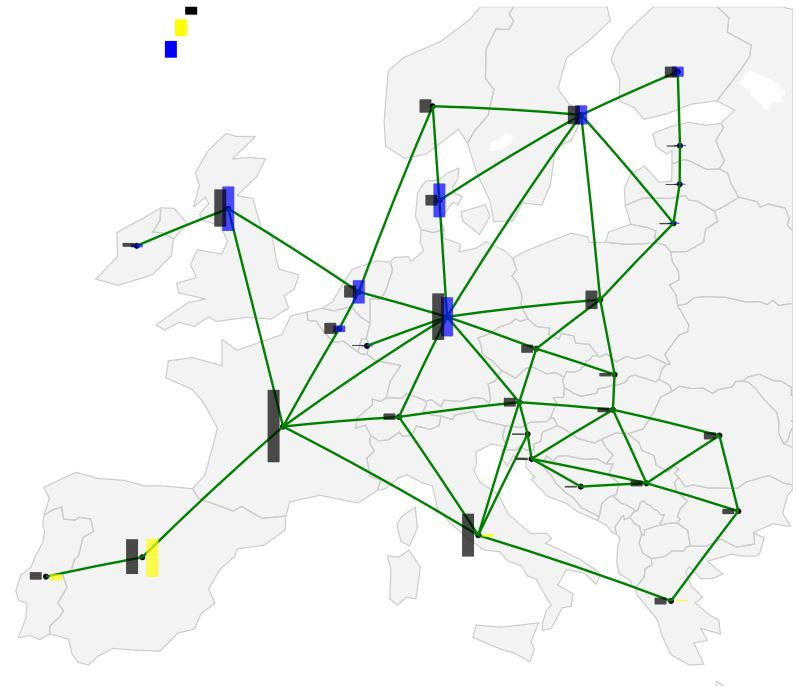
\includegraphics[width=.8\textwidth]{./Images/optimal_solution_00}
	\caption{Optimal solution for a business as usual scenario }
	\label{fig:Optimal_Solution_00}
\end{figure}

\fxnote{include demand on these plots }

\subsection{Reduced CO2 emission scenarios}


\begin{figure}[H]\centering
	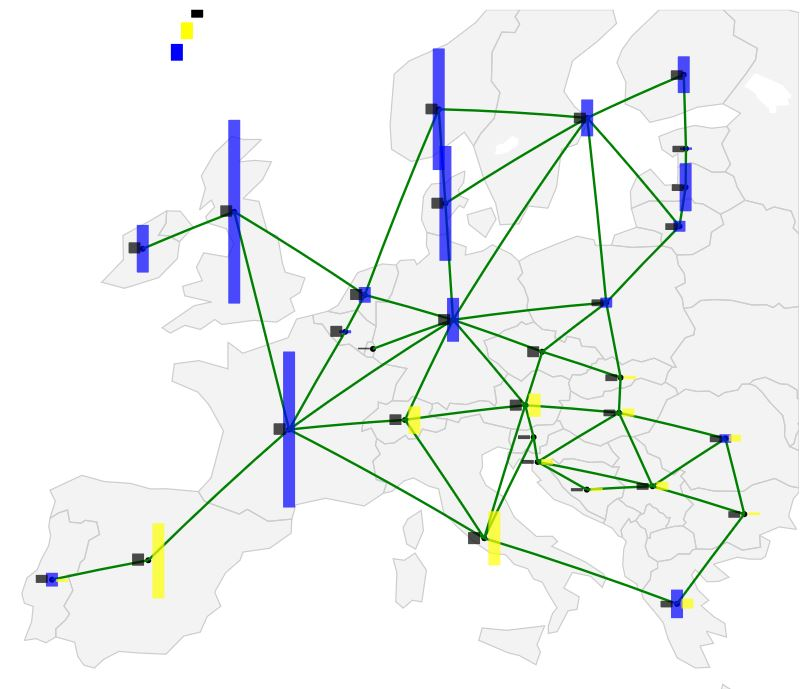
\includegraphics[width=.8\textwidth]{./Images/optimal_solution_80}
	\caption{Optimal solution for a scenario with 80\% CO2 reduction}
	\label{fig:Optimal_Solution_80}
\end{figure}

%\section{The near optimal feasible space}



\section{MGA study of grouped technologies}

In the first MGA study performed it was chosen to explore a four dimensional near optimal feasible space, with the four dimensions being total installed ocgt capacity, total installed wind capacity, total installed solar PV capacity and total installed transmission capacity. 

In the study it was found that wind energy is a key resources if CO2 emission is to be reduced by a significant amount. Analyzing figure \ref{fig:4d_hist}, showing the technology capacity distributions, it goes to show that scenarios without either wind or solar is possible in the business as usual scenario, but as soon as a CO2 constraint is implemented it is no longer possible to supply the network with electricity without a significant amount of that energy being produced by wind power. However, solar PV can in all cases of CO2 constraints be omitted. The mean solar PV capacity doeas however increase as the CO2 constraint is tightened. 

\begin{figure}[H]\centering
	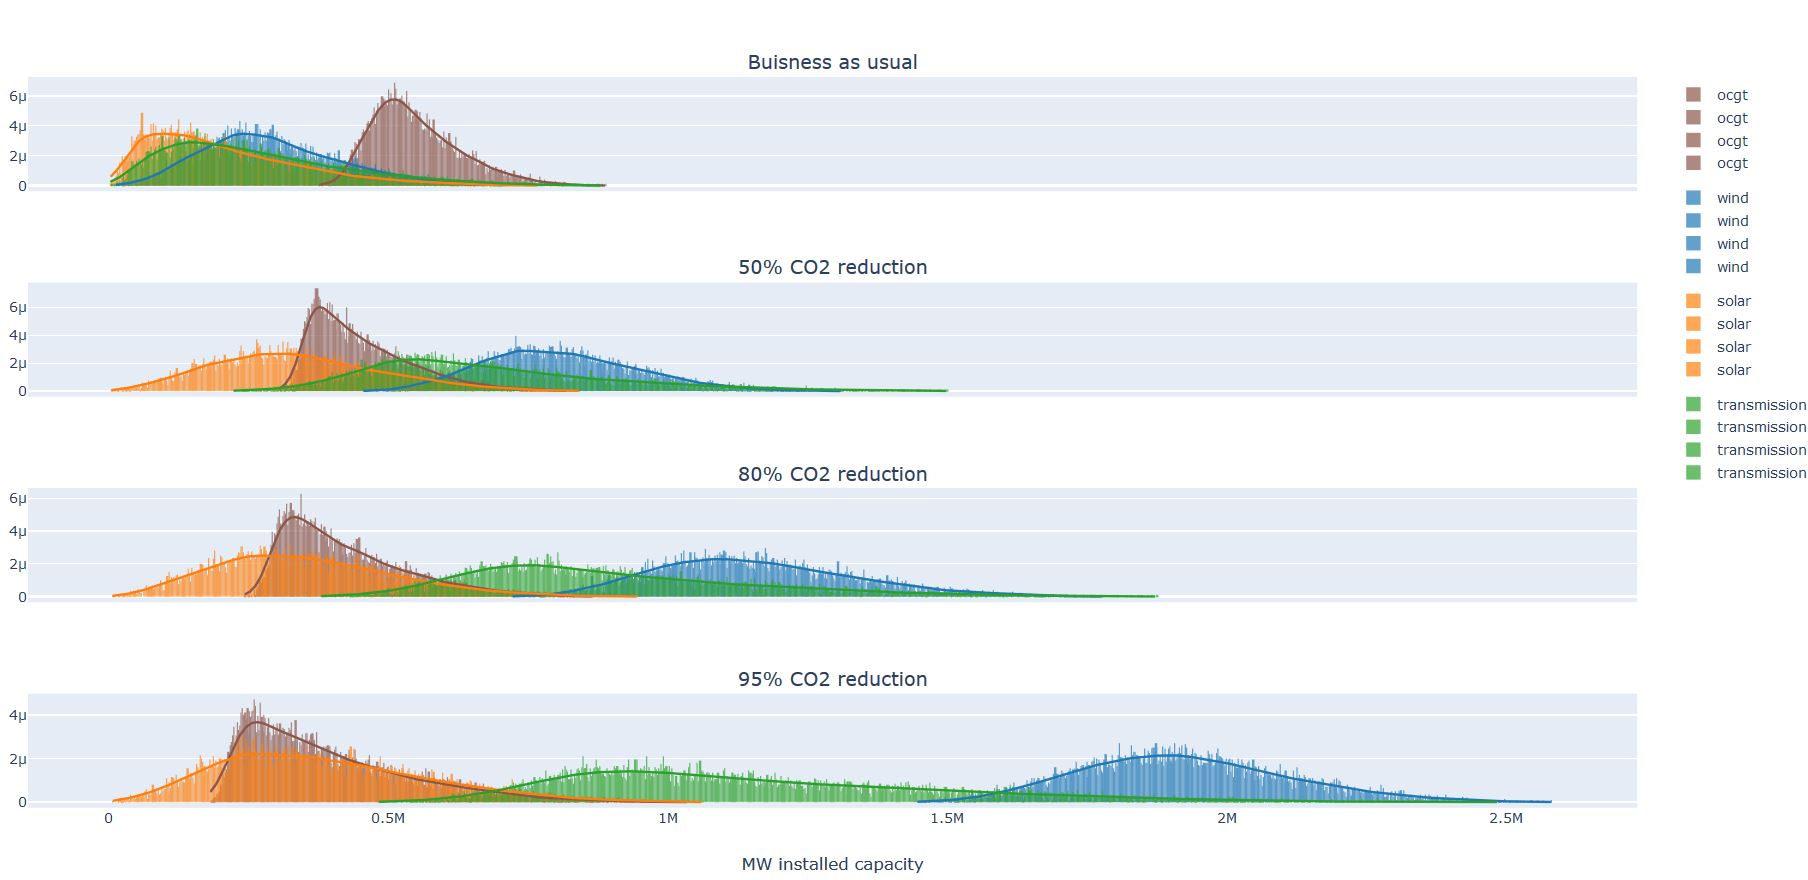
\includegraphics[width=1.\textwidth]{./Images/4D_study_histogram}
	\caption{Study of capacities with 10\% MGA slack}
	\label{fig:4d_hist}
\end{figure}

Looking at the ocgt capacities on figure \ref{fig:4d_hist}, it is clear that the distribution has a steep side towards the minimum. This indicates that there is a sharp lower limit to the amount of ocgt capacity needed in all scenarios. This minimum represents the capacity needed to supply the network with electricity, when the variable renewable energy resources are scarce. 

Furthermore, as the CO2 constraint is tightened, the deviation of all distributions increases. 


\begin{figure}[H]\centering
	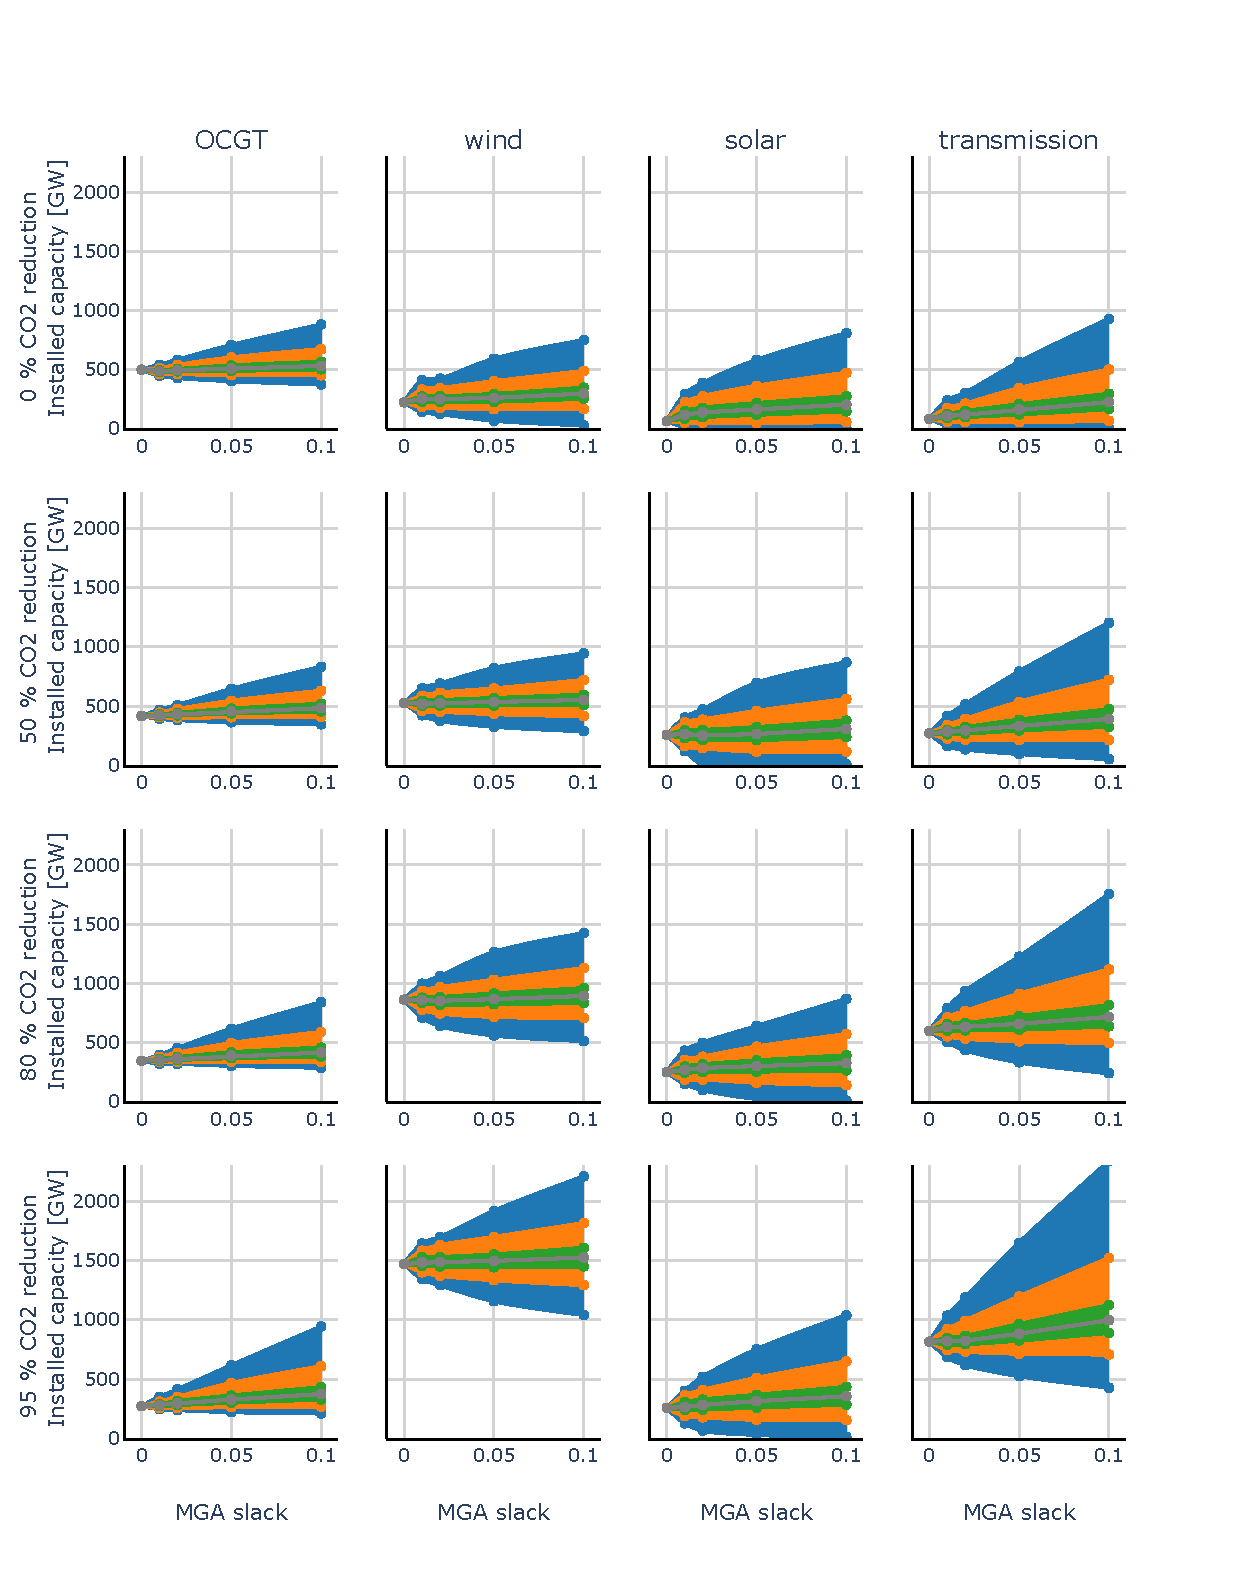
\includegraphics[width=1.\textwidth]{./Images/Capacaty_vs_cost}
	\caption{}
	\label{fig:cap_vs_cost}
\end{figure}



\section{HSJ compared to novel approach}